%%This is a very basic article template.
%%There is just one section and two subsections.
\documentclass[a4paper, ngerman]{scrartcl}

\usepackage[T1]{fontenc}
\usepackage[utf8]{inputenc}
\usepackage[ngerman]{babel}
\usepackage{lmodern}
\usepackage{amsmath}
\usepackage{amsfonts}
\usepackage{hyperref}
\usepackage{graphicx}
\usepackage{paralist}
\usepackage[none]{hyphenat}

\sloppy



\hypersetup{
pdfborder = {0 0 0},
urlbordercolor = {0 0 0},
colorlinks = true,
linkcolor = black,
citecolor = black,
filecolor = black,
urlcolor  = black
}

\title{Software-Challenge 2013 - Cartagena}
\subtitle{Spielregeln}



%% Variablen
\newcommand{\SpielSegmenteAnzahl}{\emph{5}}
\newcommand{\KartenAnzahl}{\emph{KartenAnzahl}}
\newcommand{\PiratenAnzahl}{\emph{6}}
\newcommand{\EmptyPlainPage}{\newpage\thispagestyle{plain}\ \newpage}
\newcommand{\RundenAnzahl}{\emph{15}}

\begin{document}
\parindent0px
\maketitle

\begin{figure}[h]
	\centering
	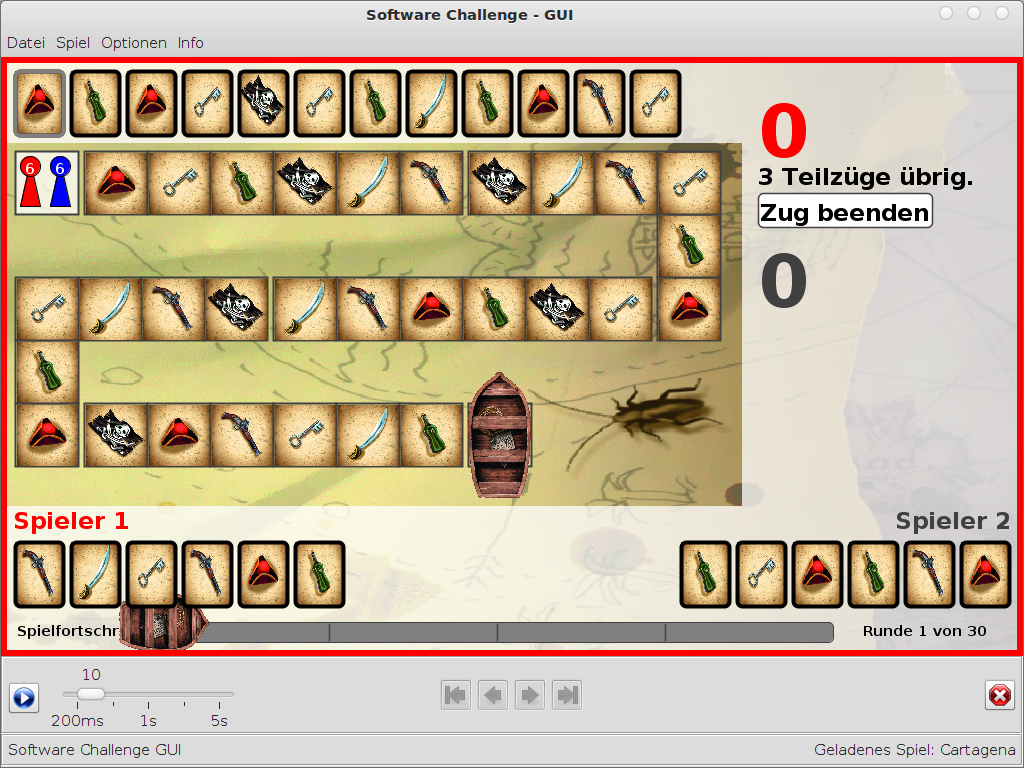
\includegraphics[width=\linewidth]{bilder/Uebersicht.png}
\end{figure}
\vspace*{\fill}
"Die Nutzung des Spielkonzeptes "Cartagena" (Name, Spielregeln und Grafik)
erfolgt mit freundlicher Genehmigung der Winning Moves Deutschland GmbH."
\newpage
\tableofcontents
\newpage

\section{Einführung}
In dieser Anleitung werden die Elemente und Regeln des Spiels \emph{Cartagena}
der Software-Challenge 2013 erläutert.\\
In dem Spiel versuchen zwei Spieler,
abwechselnd ihre Spielsteine, die Piraten, auf die Schaluppe zu bewegen. Wer
dies als Erstes schafft, gewinnt das Spiel.\\
In der implementierten Version sind jedem Spieler die nächsten 12 ziehbaren
Karten, seine eigenen, sowie die Karten des Gegners bekannt. Die
in einer Spieltaktik zu beachtenden Parameter werden dadurch um ein Vielfaches
erhöht.

\section{Spielmaterial}
	\subsection{Das Spielbrett}
Das Spielbrett setzt sich aus \SpielSegmenteAnzahl\ Segmenten zusammen,
innerhalb derer die Symbole \emph{Säbel},  \emph{Hut}, \emph{Flasche},
\emph{Flagge}, \emph{Pistole} und \emph{Schlüssel} jeweils genau einmal
vorkommen.
Die Reihenfolge ist innerhalb jedes Segmentes und von Spiel zu Spiel zufällig.
Das Spielbrett wird durch ein Start- und ein Zielfeld ergänzt.
Auf einem einzelnen Spielfeld dürfen, mit Ausnahme von Start- und Zielfeld,
jeweils maximal 3 Spielfiguren stehen. Ein mögliches Spielbrett ist in
Abbildung~\ref{fig:Spielfeld} zu sehen.


\subsection{Die Spielsteine}
Jeder Spieler startet mit \PiratenAnzahl\ Piraten im Startfeld, welche alle ins
Ziel gebracht werden müssen. Steht auf einem Spielfeld mehr als ein Pirat eines
Spielers, so wird dies durch die Zahl im Kopf der Spielfigur angezeigt.
\begin{figure}[h] \centering 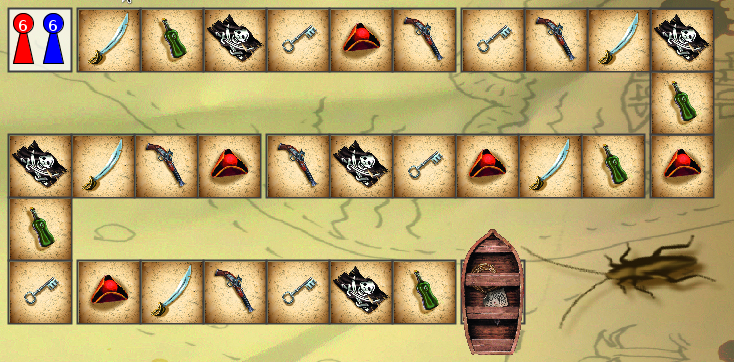
\includegraphics[scale = 0.5]{bilder/Spielfeld}
	\caption{Ein mögliches Spielbrett.}
	\label{fig:Spielfeld}
	\end{figure}
	
	\subsection{Die Spielkarten}
	
	\begin{figure}[h]
		\centering
		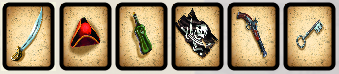
\includegraphics[scale = 0.5]{bilder/Karten}
		\caption{Die Spielkarten mit Symbolen}
		\label{fig:spielkarten}
	\end{figure}
	Zum Ziehen der Piraten werden die Spielkarten benötigt. Die Karten
	tragen analog zu den Spielfeldern wieder die Symbole \emph{Säbel},  \emph{Hut},
	\emph{Flasche}, \emph{Flagge}, \emph{Pistole} und
	\emph{Schlüssel}.\\
	Insgesamt gibt es 102 Karten, also 17 von jedem Symbol. Jeder Spieler startet
	mit 6 Karten. Er darf maximal 8 Karten besitzen.\\
	In der oberen Leiste werden die 12 Karten angezeigt, welche als
	nächstes gezogen werden können. Die Reihenfolge geht von links nach rechts.\\
	Sind alle Karten verbraucht, so werden die Karten vom (unsichtbaren)
	Ablagestapel gemischt und neu bereitgelegt.
\section{Spielablauf}	
	\begin{figure}[h]
		\centering
		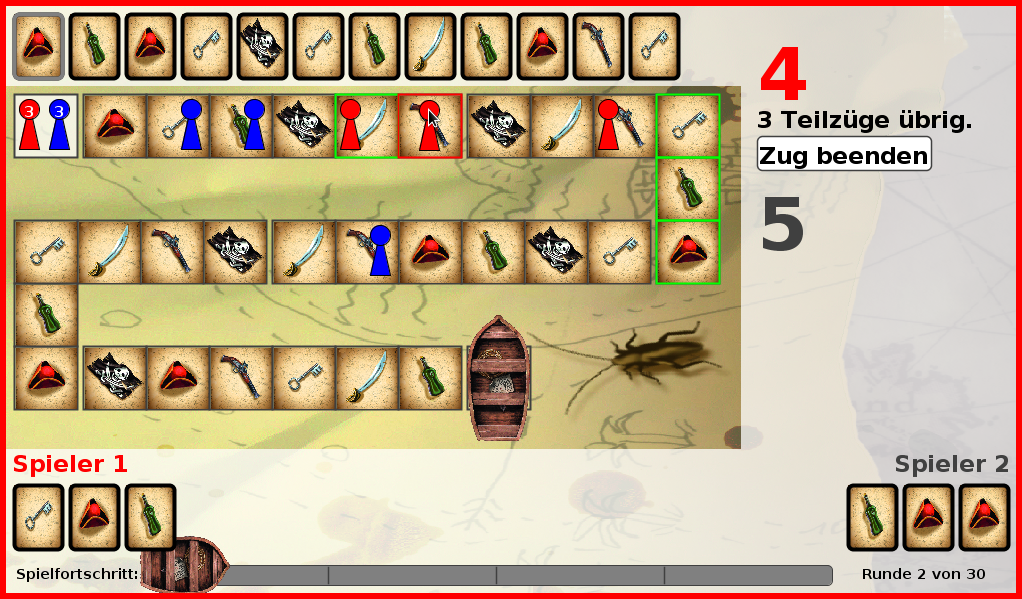
\includegraphics[scale=0.3]{bilder/Moves}
		\caption{Eine Spielsituation, in der sowohl Vorwärts- als auch Rückwärtszüge
		möglich sind.}
		\label{fig:PossibleMoves}
	\end{figure}	
	Es beginnt der rote Spieler. Jeder Spieler darf innerhalb einer Runde 3
	Teilzüge machen. Die Menge der Teilzüge darf aus einer beliebigen Kombination
	von Vorwärts- und Rückwärtszügen bestehen. Ein Spieler muss jedoch nicht alle 3
	Teilzüge nutzen, kann also auch zwei, einen oder gar keinen Teilzug tätigen.\\
	Bei einem Vorwärtszug muss der Spieler eine Karte  abgelegen, bei
	Rückwärtszügen können neue Karten vom Stapel gezogen werden.\\
	Sobald ein Spieler eine Figur ausgewählt hat, werden sämtliche Felder, auf
	welche die Figur ziehen kann, grün markiert.
	
	
	
	\subsection{Vorwärtszüge}
	Bei einem Vorwärtszug wählt ein Spieler eine seiner
	Spiel\-figuren. Zum Vorwärtsziehen muss eine Karte
	abgelegt werden und die Spielfigur zieht auf das nächste unbesetzte Feld,
	welches das gleiche Symbol wie die Karte zeigt. Alle übrigen Felder sowie
	einfach oder mehrfach besetzte Felder werden hierbei übersprungen.\\
	Gibt es zwischen einem Piraten und der Schaluppe kein Feld mehr mit dem auf
	einer Karte abgebildeten Symbol oder sind alle Felder mit diesem Symbol
	belegt, so kann durch Ablegen dieser Karte direkt auf das Zielfeld gezogen
	werden. In der Implementierung geschieht dies durch Ziehen einer Spielfigur auf
	das Zielfeld. Gibt es mehrere Kartensymbole, welche abgelegt werden können, so
	werden die betreffenden Karten grün markiert. Durch Anklicken einer Karte wird
	diese dann genutzt, um auf das Zielfeld zu ziehen.
	
	\begin{figure}[h]
		\centering
		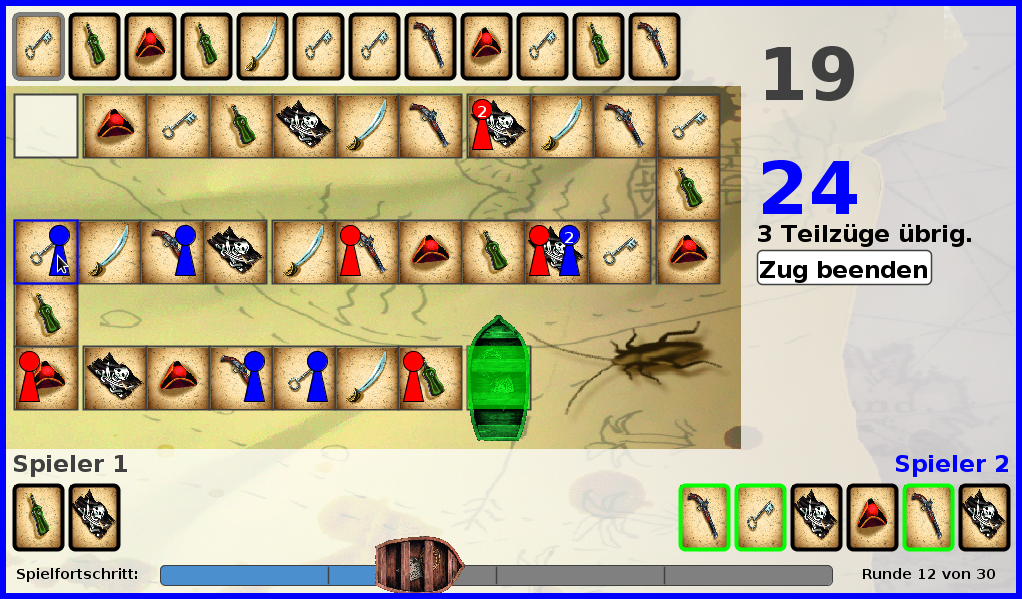
\includegraphics[scale = 0.3]{bilder/zielfeld}
		\caption{Durch Ablegen einer Pistole oder des Schlüssels kann der blaue
		Spieler den ausgewählten Piraten (blau umrandet) ins Zielfeld bewegen.}
		\label{fig:Zielfeld}
	\end{figure}
	 
\subsection{Rückwärtszüge}
Durch Rückwärtszüge können neue Karten aus dem offen liegenden Kartenvorrat
gezogen werden.
Hierbei wählt ein Spieler eine Spielfigur aus und zieht sie auf das nächste
zurückliegende Feld, auf dem bereits mindestens eine und höchstens zwei
Spielfiguren stehen. Das Startfeld ist hierbei ausgeschlossen und es ist egal,
welche Farbe die Spielsteine auf dem zurückliegenden Feld haben. Auch wenn eine
Spielfigur schon auf dem Zielfeld steht, kann diese wieder zurück bewegt
werden.\\
Stehen auf dem zurückliegenden Feld 2 Piraten, so zieht der Spieler 2 neue
Karten, sonst darf er nur eine Karte ziehen. Die Karten werden dabei jeweils von
links gezogen. Hat ein Spieler schon 8 Karten, so werden keine neuen Karten
gezogen.\\
Stehen auf dem nächsten zurückliegenden Feld bereits 3 Spielsteine, darf auf
dieses Feld nicht gezogen werden. Beim Zurückziehen muss dieses Feld dann
übersprungen werden.\\
Neu dazugekommene Karten werden immer
Richtung Bildmitte positioniert. Die neuen Karten des roten Spielers befinden sich also ganz rechts in seiner
Kartenanzeige, die des blauen Spielers ganz links.



\subsection{Spezialfall: Keine Züge möglich}
	
	Sollte der Fall eintreten, dass ein Spieler keine Karten besitzt und keine
	Rückwärtszüge möglich sind, so muss dieser Spieler aussetzen bzw. einen leeren
	Zug senden (siehe Abbildung ~\ref{fig:zugunfaehig}).
	\begin{figure}[h]
	 \centering
	 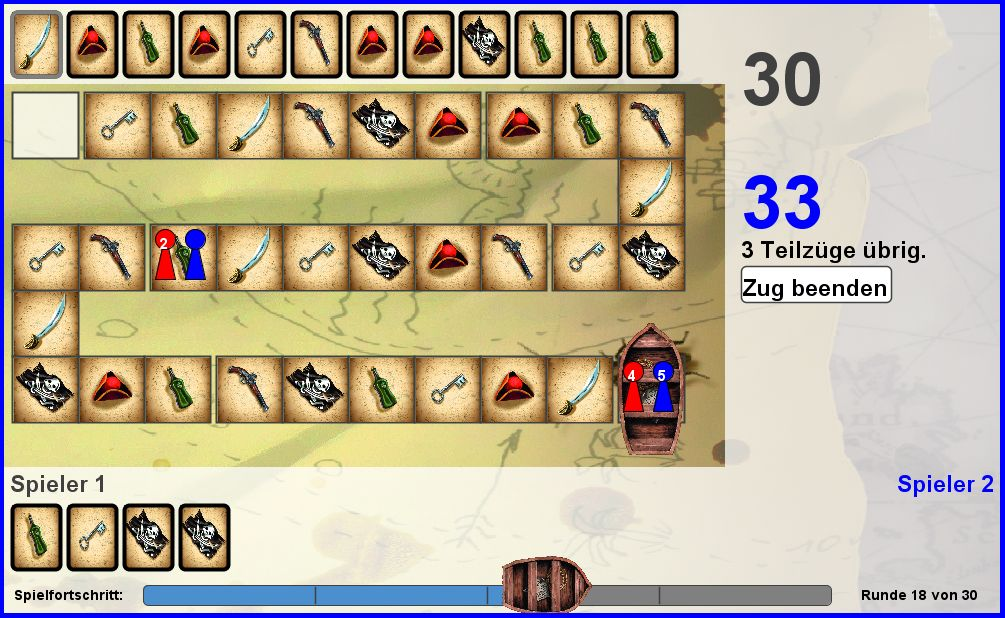
\includegraphics[scale = 0.3]{bilder/zugunfaehig}
	 \caption{Der blaue Spieler ist zugunfähig. Er muss eine Runde aussetzen.}
	 \label{fig:zugunfaehig}
	\end{figure}
	
	\subsection{Punkteverteilung}
	Die Punkte ergeben sich aus der Anzahl der Piraten, welche sich im jeweiligen
	Segment befinden. Hat ein Spieler beispielsweise zwei Piraten in Segment 1 und
	einen Piraten in Segment 3, so ergibt sich eine Gesamtpunktzahl von 5.\\
	Spielsteine auf dem Startfeld bringen keine Punkte und ein Pirat im Zielfeld
	bringt 6 Punkte.
	
\section{Ende des Spiels}

	Hat ein Spieler alle seine Piraten im Zielfeld, so gewinnt dieser. Schafft dies
	keiner der beiden Spieler innerhalb der \RundenAnzahl\ Runden, so
	gewinnt der Spieler mit den meisten Punkten.
	
\section{Die graphische Benutzeroberfläche}
\subsection{Übersicht der graphischen Benutzeroberfläche}
	In Abbildung~\ref{fig:GUI} ist ein Überblick der graphischen Benutzeroberfläche
	zu sehen. Die markanten Spielelemente sind mit \emph{a-e} gekennzeichnet.
	
	 \begin{figure}[h!]
		\centering		
		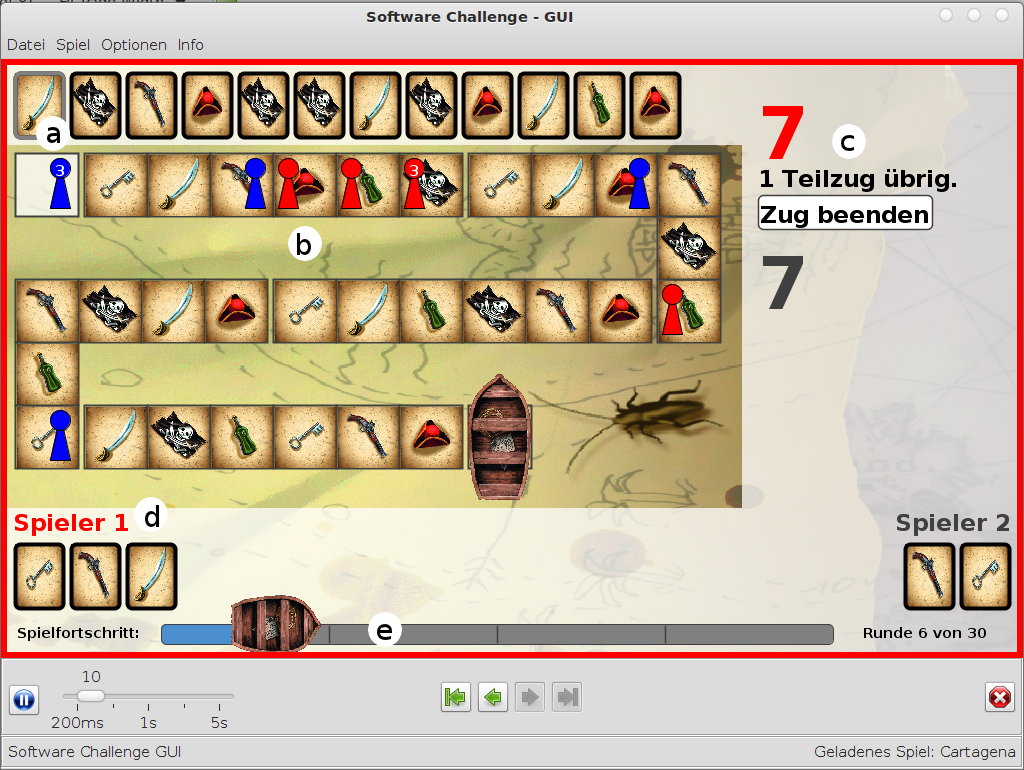
\includegraphics[scale = 0.3]{bilder/gui}
		\caption{Überblick der GUI}
		\label{fig:GUI}
	\end{figure}
	
\begin{compactenum}[a)] \item Die nächsten ziehbaren Karten. Die Erste befindet
sich links.
\item Das Spielbrett \item Punkteanzeige, Anzeige der verbleibenden Züge und
Button, um einen Zug vorzeitig zu beenden. Die Punkte des roten Spielers sind
oben, die des blauen Spielers unten. Die Punkte des inaktiven Spielers sind
jeweils immer grau.
\item Die Karten von Spieler 1. Neu dazugekommene Karten werden immer Richtung
Bildmitte positioniert.
\item Spielfortschrittsanzeige
	\end{compactenum}
	
\subsection{Das Einstellungsmenü}
	 \begin{figure}[h]
		\centering
		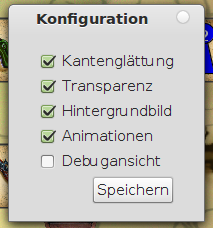
\includegraphics[scale=0.5]{bilder/configuration}
		\caption{Das Einstellungsmenü}
		\label{fig:Configuration}
	\end{figure}
	
	Ein Einstellungsmenü mit Darstellungsoptionen lässt
sich über die Leertaste anzeigen. Dazu muss das
Spielfeld den Tastaturfokus haben (erforderlichenfalls
vorher Mausklick auf das Spielfeld). Es stehen dort
folgende Einstellungen zur Verfügung:

\textbf{Kantenglättung} und \textbf{Transparenz} verbessern die Optik des
Spiels, sind aber rechenintensiv. Auf sehr langsamen Rechnern sollten sie daher
deaktiviert werden. \textbf{Hintergrundbild} ist zwar weniger rechenintensiv,
kann aber auch aus Gründen der Übersichtlichkeit deaktiviert werden.\\
\textbf{Animationen} legt fest, ob die Bewegungen der Spielsteine in
Wiederholungen und bei Computerspielern animiert werden sollen.\\
Die \textbf{Debugansicht} verkleinert die Punkteanzeige in der Seitenleiste
etwas und zeigt unterhalb Debug-Hilfestellungen zu einzelnen Zügen an. Diese
Hilfestellungen sind Texte, die ein Spielclient einem Zug beifügen kann, den er
an den Spielserver sendet.
	
\end{document}
